% !TEX root =  master.tex
\section{User-Journey}
\label{sec:user_journey}
Anhand der nun weitestgehend geschilderten Anforderungen aller Personas wurde der Aufbau der Website für das entwickelte Kinobuchungssystem entschieden.
Diese gewählte Struktur wird im Folgenden anhand eines Beispiels geschildert, in welchem ein Endnutzer drei Tickets für eine spezielle Filmvorführung bucht.
Vorausgesetzt ist hierbei, dass der Nutzer tatsächlich eine Online-Buchung vornimmt und nicht direkt im Kino anruft, um ein Ticket zu erwerben bzw. einen Sitzplatz zu reservieren.

\begin{figure}[ht]
	\centering
	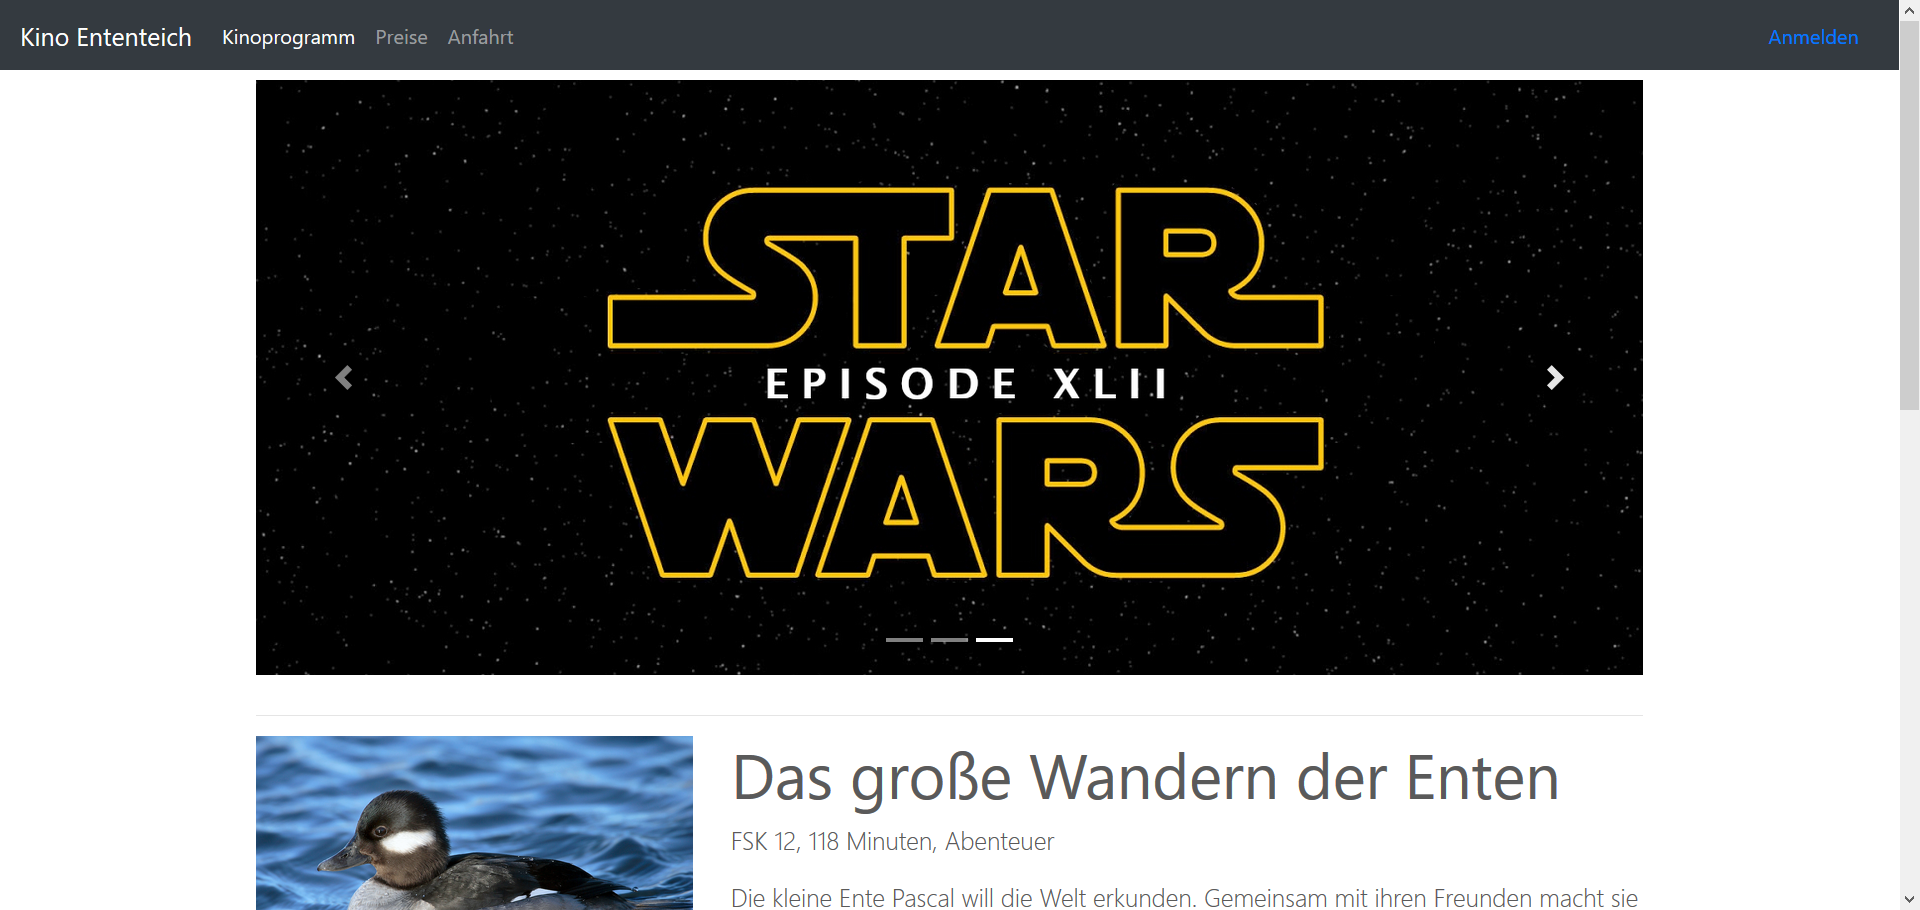
\includegraphics[width=\textwidth]{img/screenshots/startseite00}
	\captionsetup{format=hang}
	\caption{Startseite}
	\label{fig:startseite00}
\end{figure}

Bei Aufruf der Startseite des Kinos wird dem Nutzer eine Übersicht über alle momentan im Kino laufenden Filme präsentiert.
Ganz oben befindet sich dabei ein Karussell mit den beliebtesten Filmen.
Darunter ist eine Liste mit allen Filmen.
Durch Herauf- und Herabscrollen lässt sich schnell durch diese Liste navigieren, das Finden des gesuchten Films wird durch die großen Cover-Bilder neben dem Titel erleichtert.
Durch Anwählen des Filmtitels wird der Nutzer auf die Seite für diesen Film geleitet, auf der alle Vorstellungen des Films innerhalb der nächsten Tage aufgelistet sind.
Dort findet sich auch eine detaillierte Beschreibung und eine Bewertung des Films durch andere Benutzer (vgl. Anhang \vref{sec:screenshots_frontend}).

Eine jede dieser Vorstellungen ist durch einen Knopf in der nach Tagen geordneten Tabelle repräsentiert, mit der passenden Uhrzeit als Beschriftung.
Wurde der Knopf mit dem gewünschten Vorstellungszeitpunkts ausgewählt, so wird der Nutzer zur Sitzplatzübersicht und -auswahl weitergeleitet.

Als nächstes ist für den Anwender die Wahl der Sitzplätze relevant.
Dies geschieht im entwickelten Buchungssystem durch die Anwahl der Plätze in einer 2D-Grafik des Kinosaals, in welcher bereits belegte, freie und eigens angewählte Plätze farblich voneinander abgehoben sind.
Nach der Auswahl der gewünschten Sitzplätze sollte der Nutzer nun in der Lage sein, die Preiskategorien der Plätze (Ermäßigungen usw.) auszuwählen und den Einzel- sowie Gesamtpreis der Auswahl einsehen zu können.

\begin{figure}[ht]
	\centering
	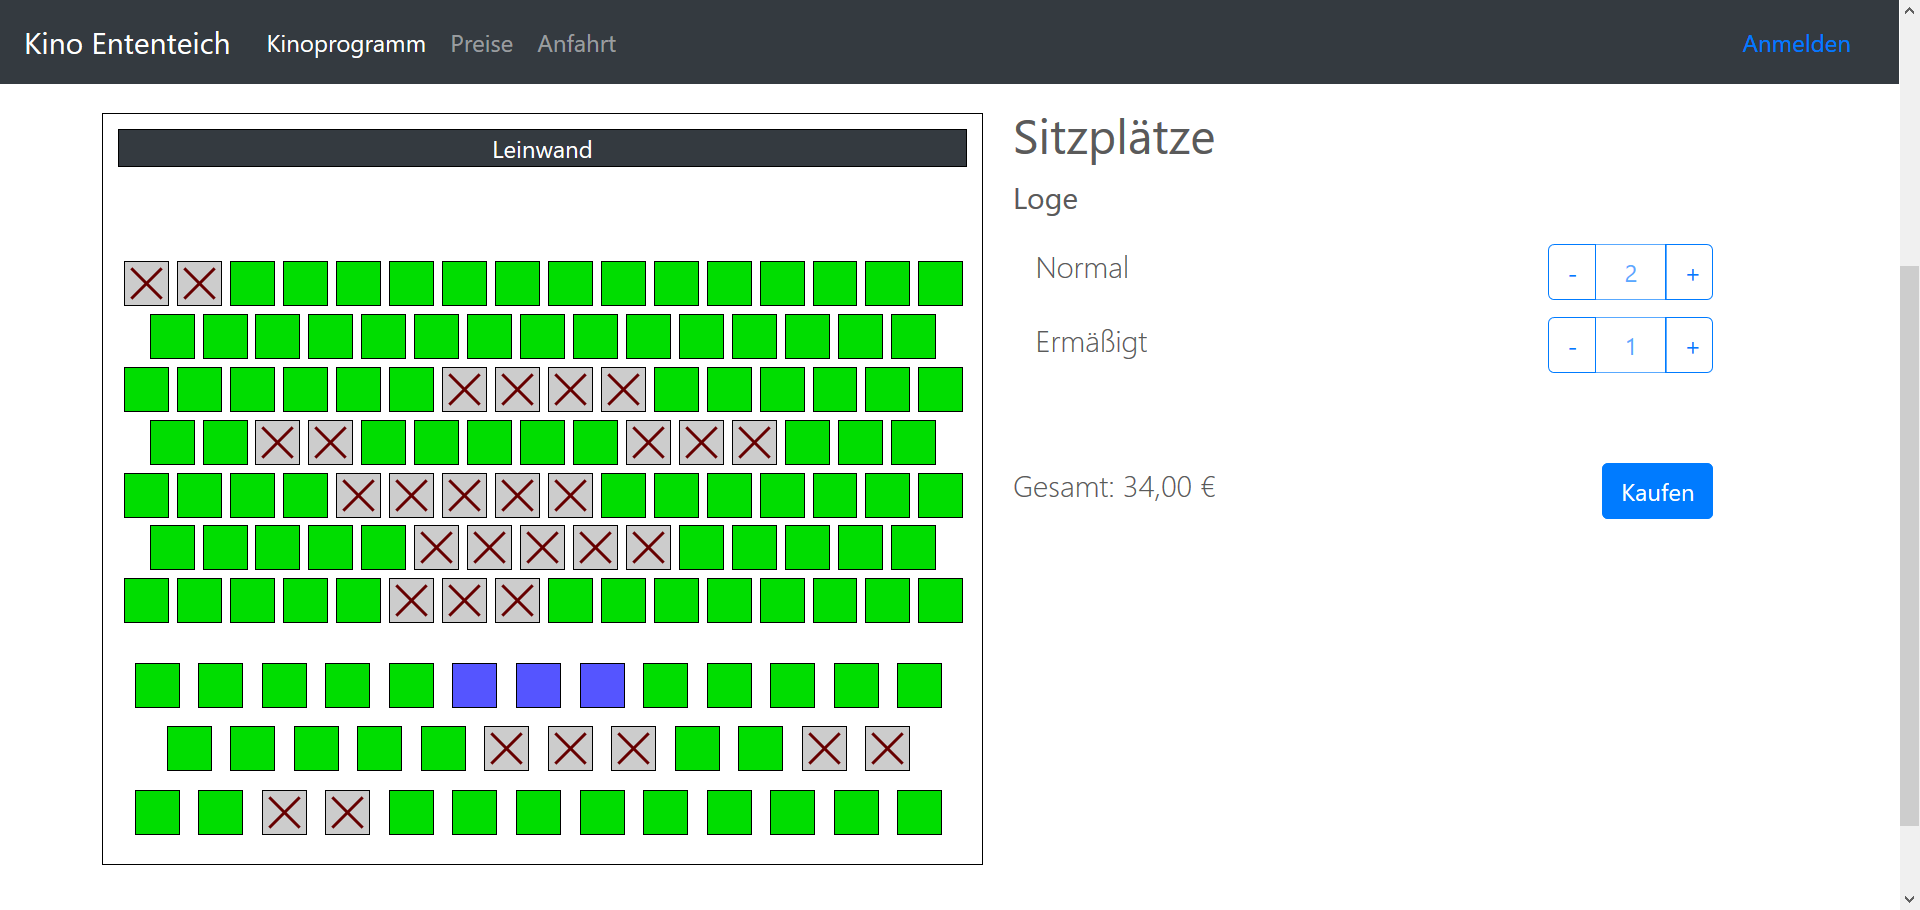
\includegraphics[width=\textwidth]{img/screenshots/vorstellung02}
	\captionsetup{format=hang}
	\caption{Auswahl der Sitzplätze}
	\label{fig:vorstellung02-2}
\end{figure}

Ist der Nutzer mit diesem Schritt fertig, kommt es nun zum Bezahlvorgang für die ausgewählten Tickets.
Hier soll der Nutzer eine kompakte Übersicht über die Bestellung erhalten, und nach Überprüfung seiner Auswahl seine persönlichen Daten (Vorname, Nachname und E-Mail-Adresse) angeben können.
Drüber hinaus soll noch die Auswahl zwischen mehreren Zahlungsmethoden sowie die Eingabemöglichkeit für Rabattcodes angeboten werden.

Mit der Zahlungsbestätigung ist der Nutzer im letzten Schritt des Buchungsvorgangs angelangt.
Hier werden erneut die zusammengefassten Details der Bestellung (Kosten, Sitzplätze, Filmdetails und Vorstellungszeitpunkt) sowie ein Bestätigungstext angezeigt.
Außerdem wird dem Nutzer sein digitales Ticket in Form eines \acs{QR-Code}s angezeigt, welches der Anwender auch per E-Mail zugesandt bekommt oder mithilfe eines Accounts in der mobilen App abrufen kann.
Dieser Code enthält alle Infos über das Ticket und ist im Kino gleichwertig mit einer ausgedruckten Version.

Neben diesem Anwendungsfall gibt es natürlich noch andere Berührungspunkte der Anwender mit dem System außerhalb der Aufgabenstellung dieser Arbeit.
Hierzu zählen unter anderem eine Ticketbuchung bzw. -reservierung per Telefon sowie die Verarbeitung einer Buchung durch einen Kinomitarbeiter.
Im Allgemeinen ähneln sich die Schritte insofern, dass Film-, Vorstellungs- und Sitzplatzauswahl vom Ablauf her gleich bleiben, für den Kinomitarbeiter jedoch kompakter dargestellt werden können.
Filmbeschreibungen, Bewertungen, Titelbilder usw. spielen hier keine Rolle, da diese Informationen für den Mitarbeiter als Fachmann irrelevant sind.